% ============================================
\section{Przegląd modułów}
% ============================================

\subsection{Moduł I --- Podstawowe dane}

\begin{frame}[t]{Moduł I}{Podstawowe dane}
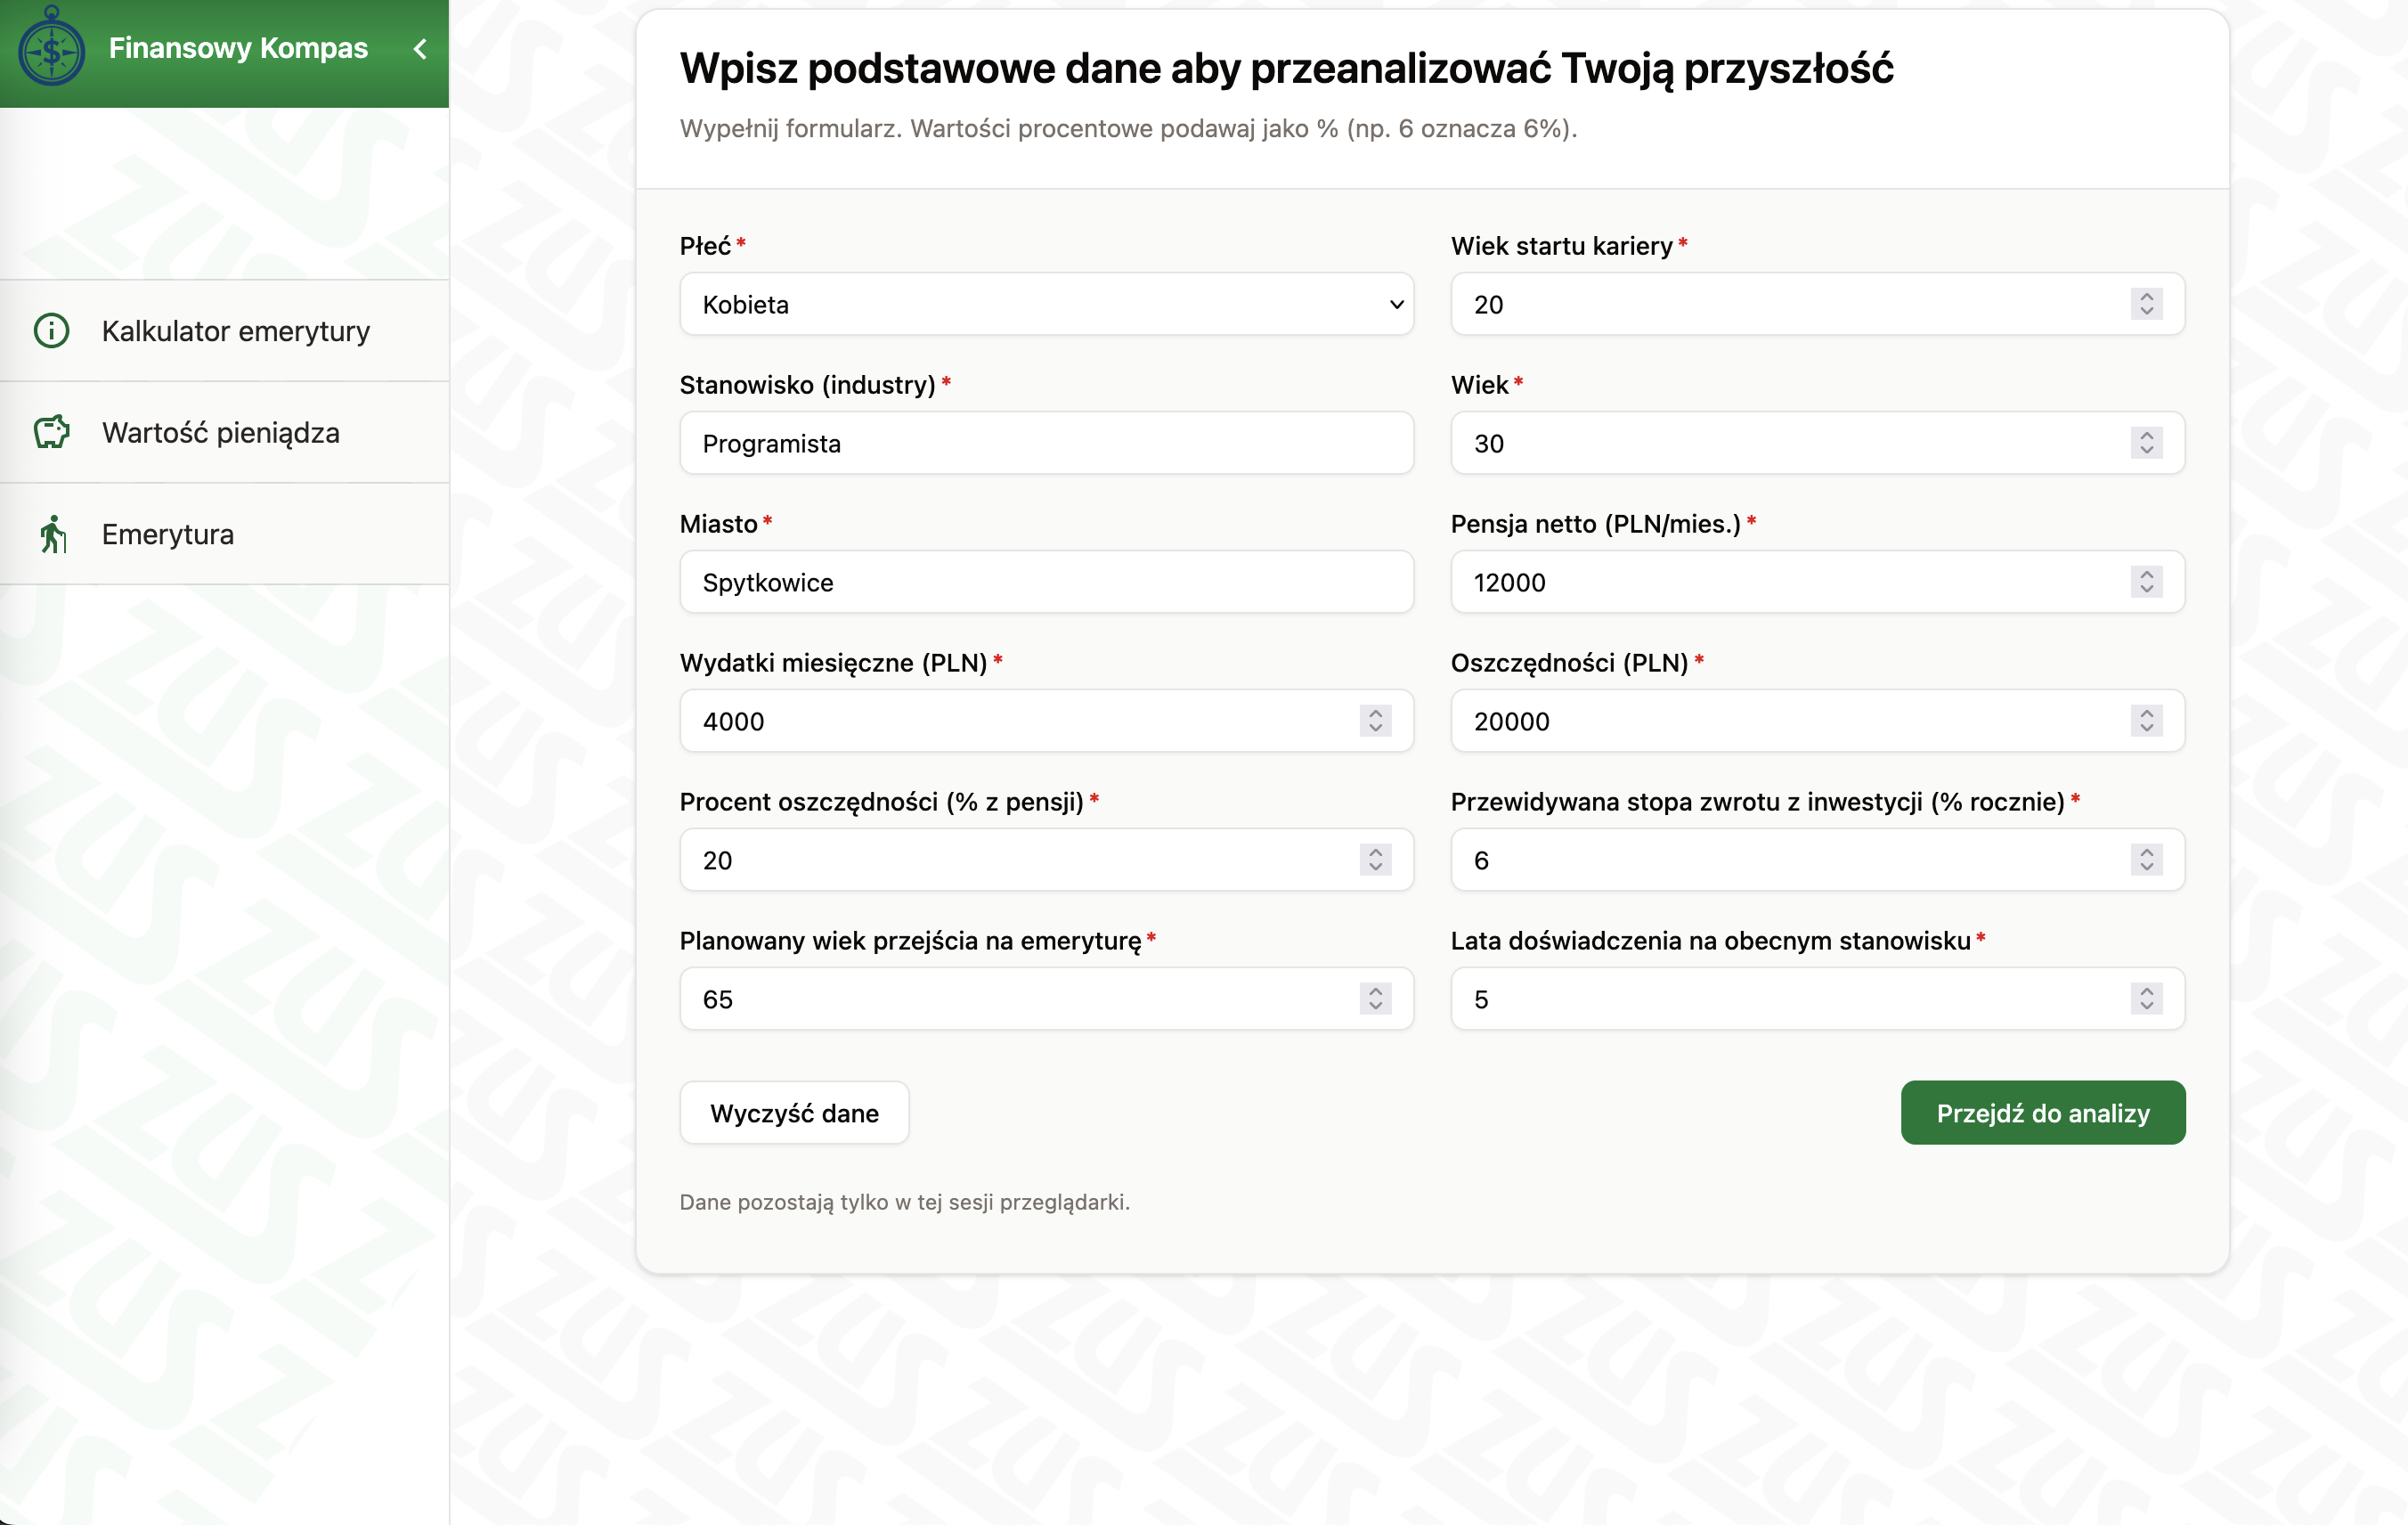
\includegraphics[width=.8\textwidth]{img/module_1_basic_data}
\end{frame}

\begin{frame}[t]{Moduł I}{Podstawowe dane}
    Przy minimalnym zestawie danych pochodzących od użytkownika:
    \pause
    \begin{itemize}
    \item zawód/branża
    \pause
    \item miejscowość zamieszkania
    \pause
    \item wiek
    \end{itemize}
    \pause
    Nasz system od razu wylicza model finansowy dla użytkownika:
    \begin{itemize}
    \pause
        \item projekcję wynagrodzeń w przyszłości (nominalnych i realnych)
    \pause
        \item miesięczne wydatki, oszczędności, lata doświadczenia na stanowisku, wiek przejścia na emeryturę
\pause --- wszystkie wartości mogą zostać poprawione i uszczegółowione przez użytkownika w każdej chwili
    \end{itemize}
\end{frame}

\subsection{Moduł II --- Uproszczony kalkulator emerytalny}

\begin{frame}[t]{Moduł II}{Uproszczony kalkulator emerytalny}
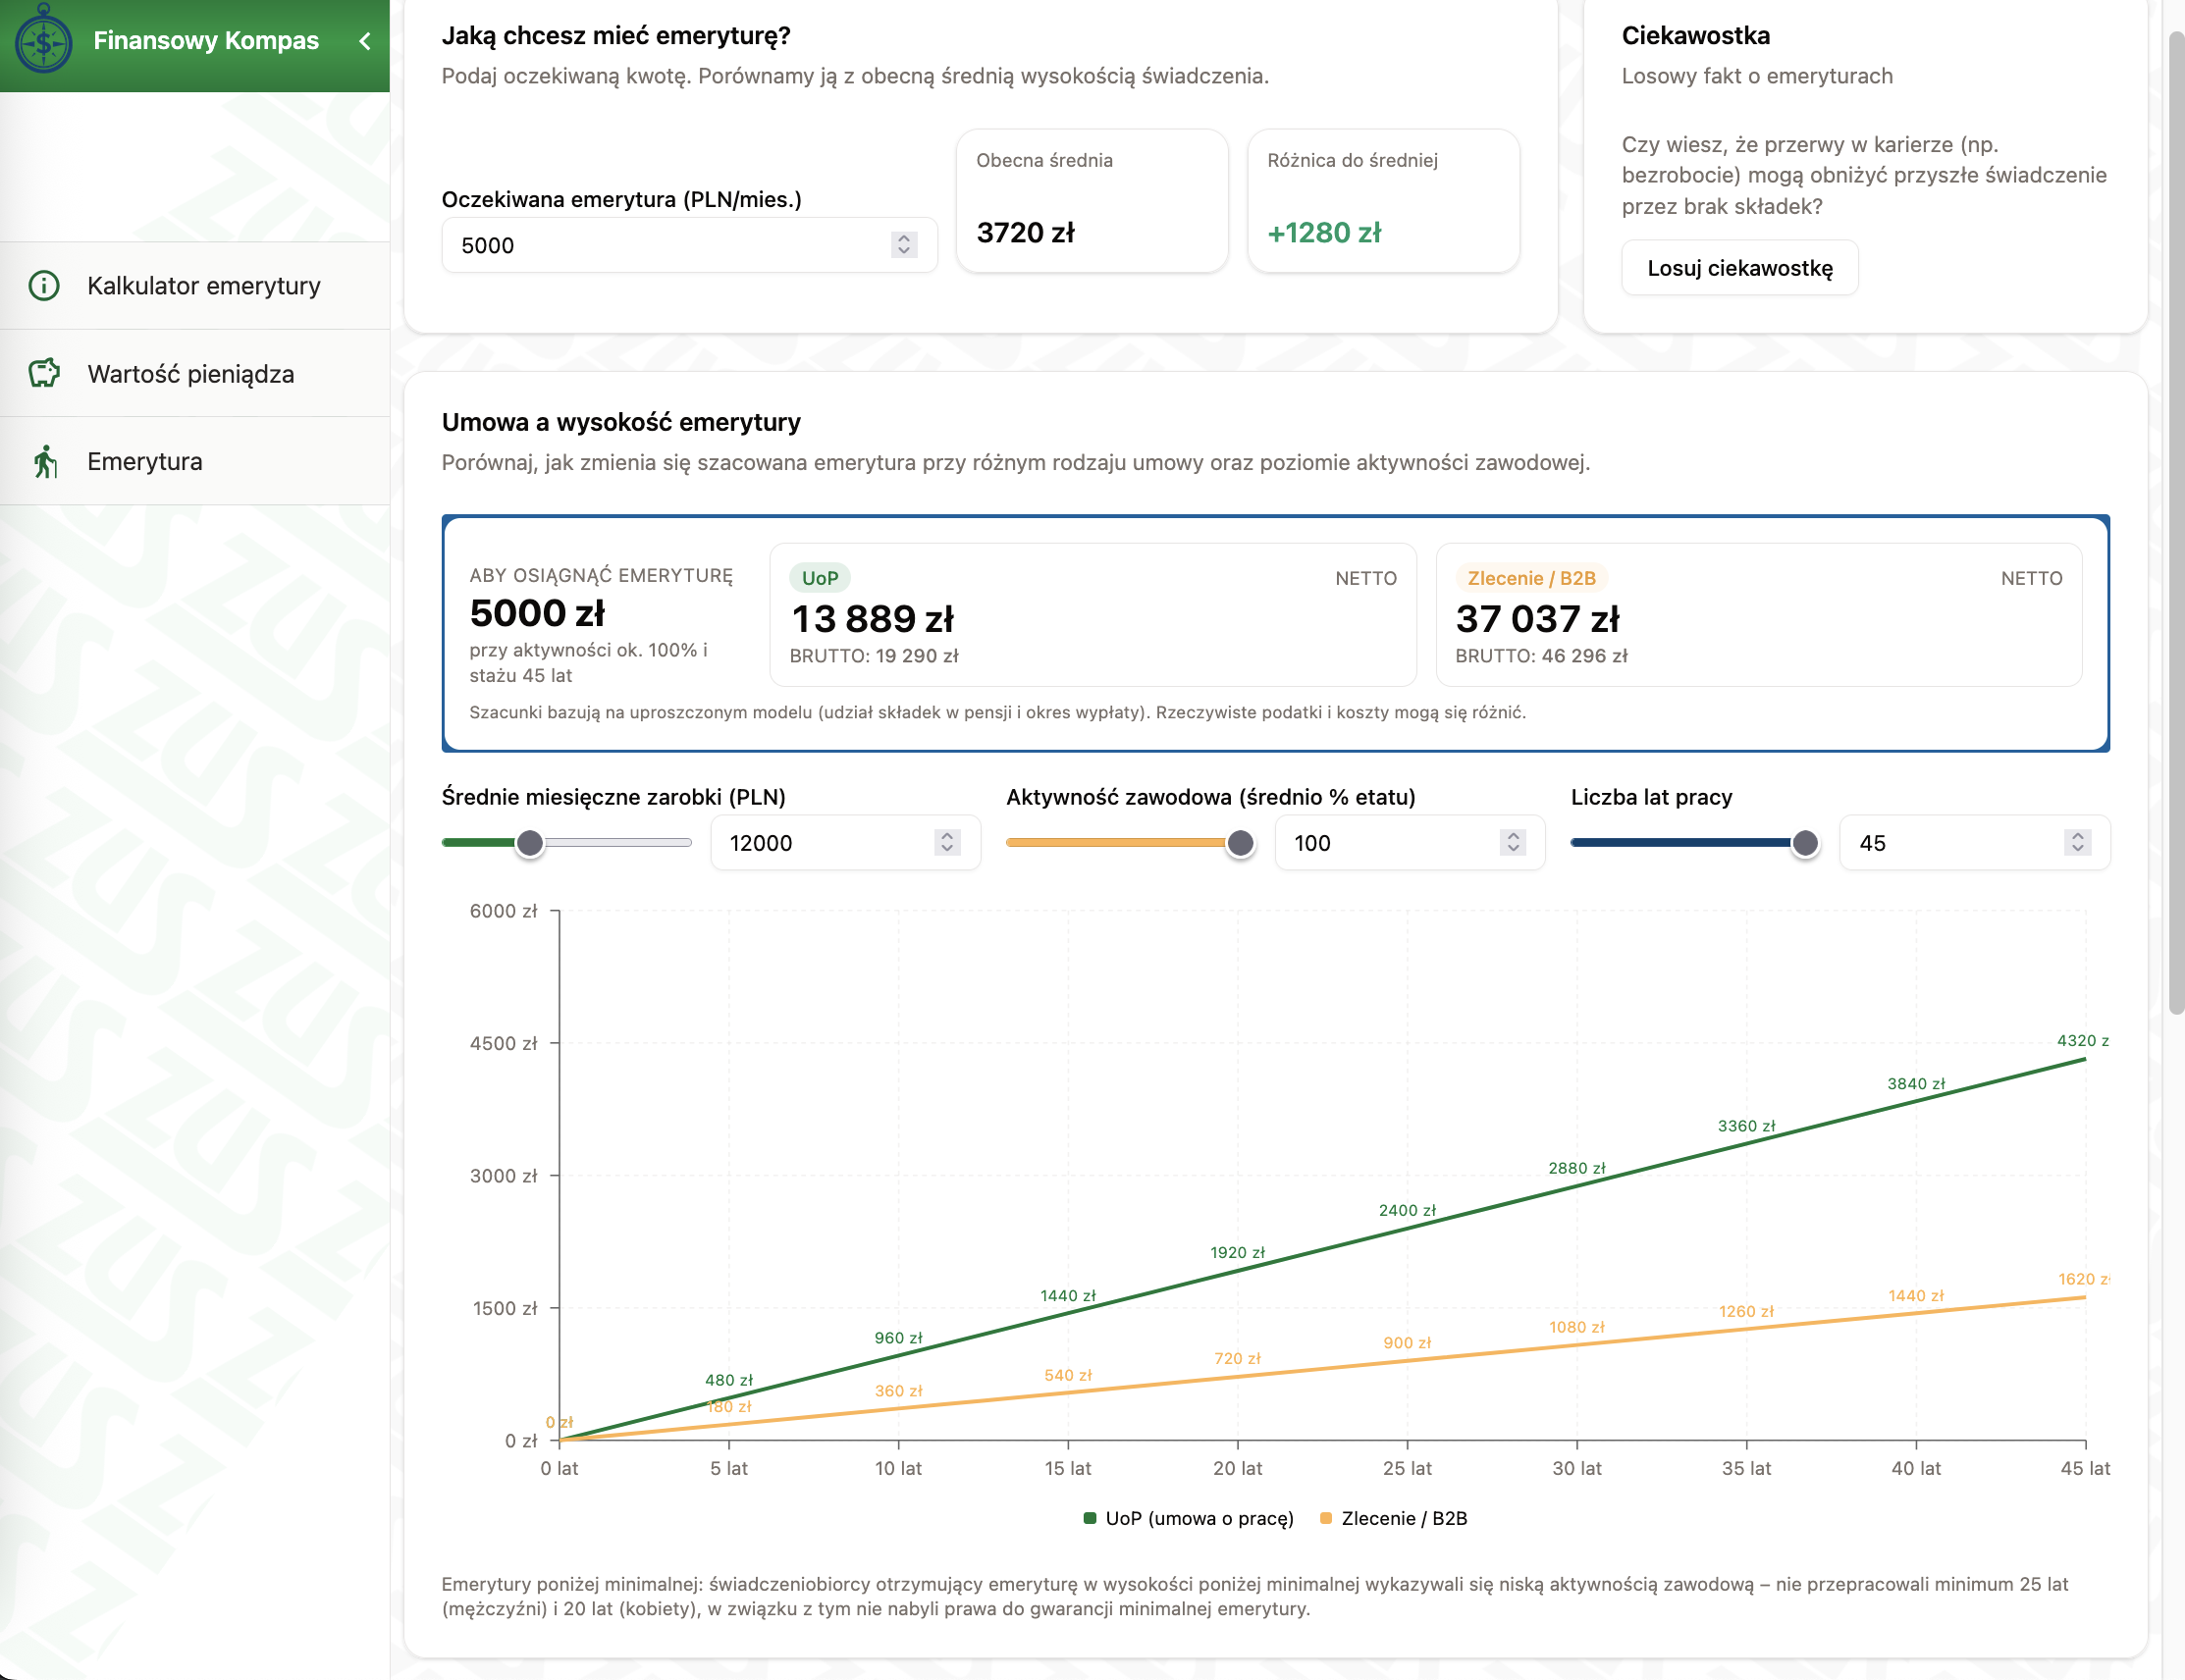
\includegraphics[width=.8\textwidth]{img/module_2_simple_pension_calculator}
\end{frame}

\begin{frame}[t]{Moduł II}{Uproszczony kalkulator emerytalny}
    Dynamiczny wykres ilustrujący zależność między planowaną emeryturą nominalną,
    a charakterystyką historii zatrudnienia użytkownika: średnimi zarobkami,
    stażem aktywności zawodowej i wymiarem etatu.
\end{frame}


\begin{frame}[t]{Moduł II}{Uproszczony kalkulator emerytalny}
Moduł pozwala też porównać emeryturę dla pracownika zatrudnionego na warunkach umowy o pracę w kontrze do osoby
prowadzącej tzw. Jednoosobową Dzialalność Gospodarczą (B2B), przy zalożeniu minimalnego, zgodnego z przepisami
wkładu do ZUS.
\end{frame}

\begin{frame}[t]{Moduł II}{Uproszczony kalkulator emerytalny}
Moduł oferuje też dynamicznie pobierane informacje w formie ciekawostek, które realizują cel
subtelnego edukowania naszej grupy docelowej --- młodych użytkowników --- o różnych aspektach
polskiego systemu emerytalnego.
\end{frame}

\begin{frame}[t]{Moduł II}{Uproszczony kalkulator emerytalny}
Inną formą ciekawostek serwowanych w tym module jest wreszcie wykres ilustrujący
medianę emerytury dla dziesięciu losowo wybranych zawodów.
\\[2em]
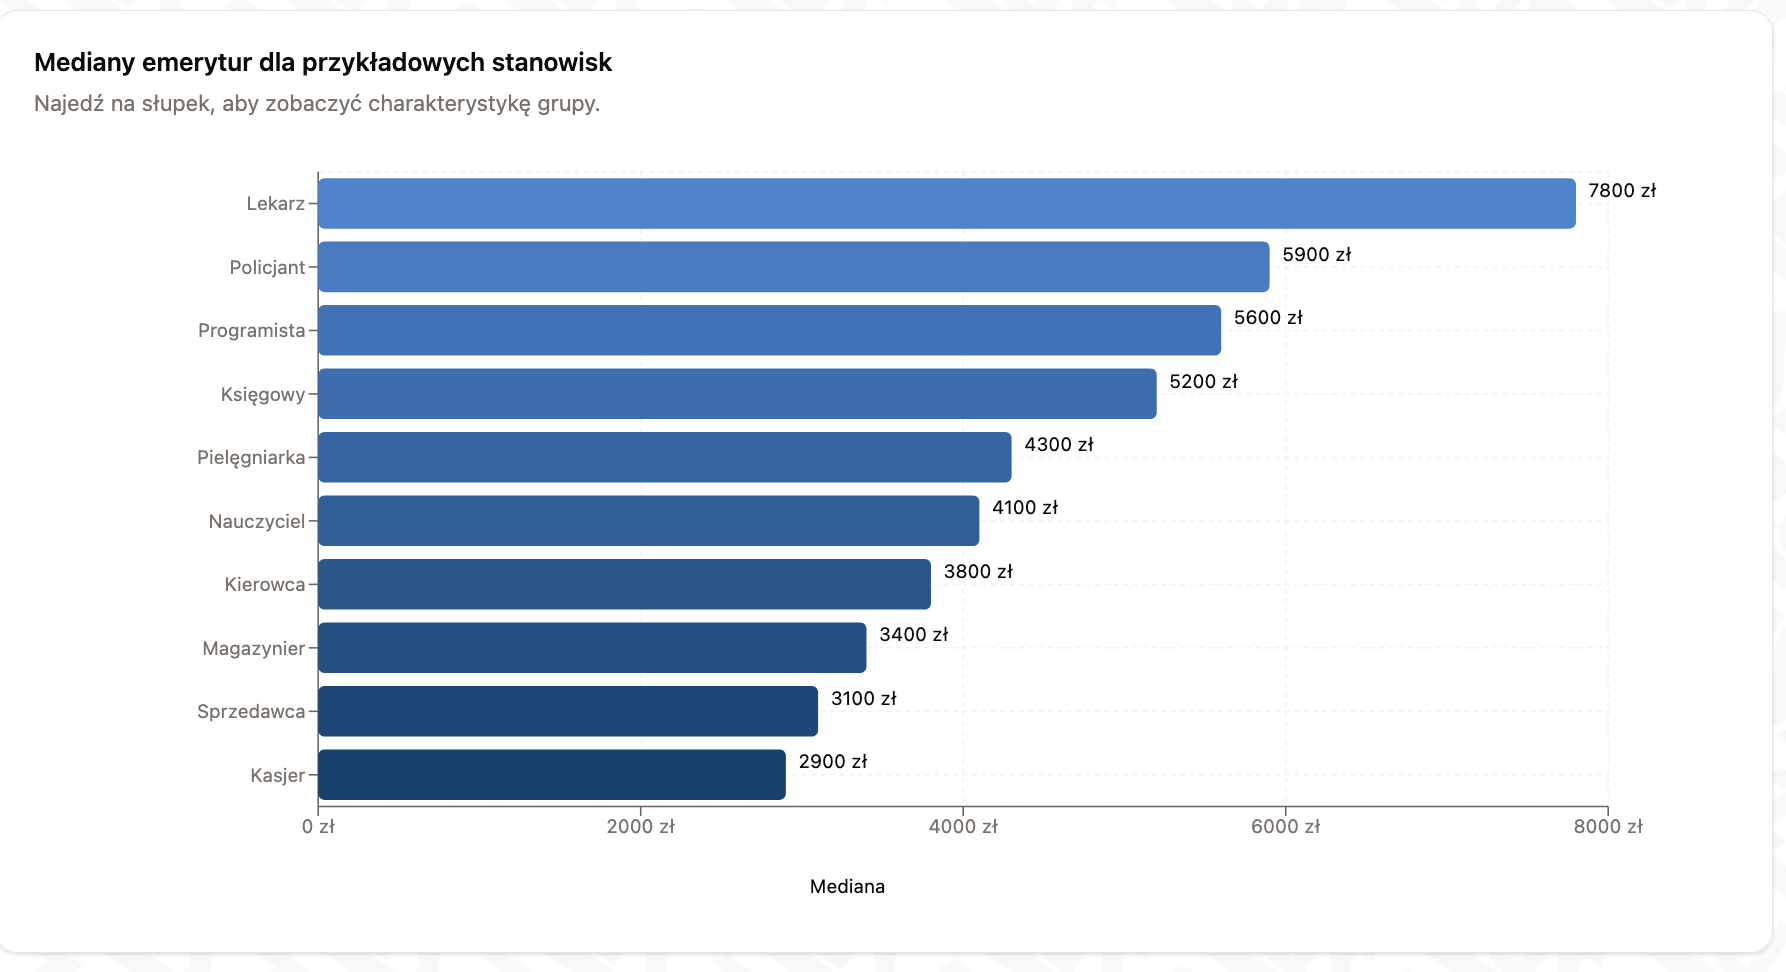
\includegraphics[width=.8\textwidth]{img/module_2b_median_pensions}
\end{frame}

\subsection{Moduł III --- Wartość pieniądza}

\begin{frame}[t]{Moduł III}{Wartość pieniądza}
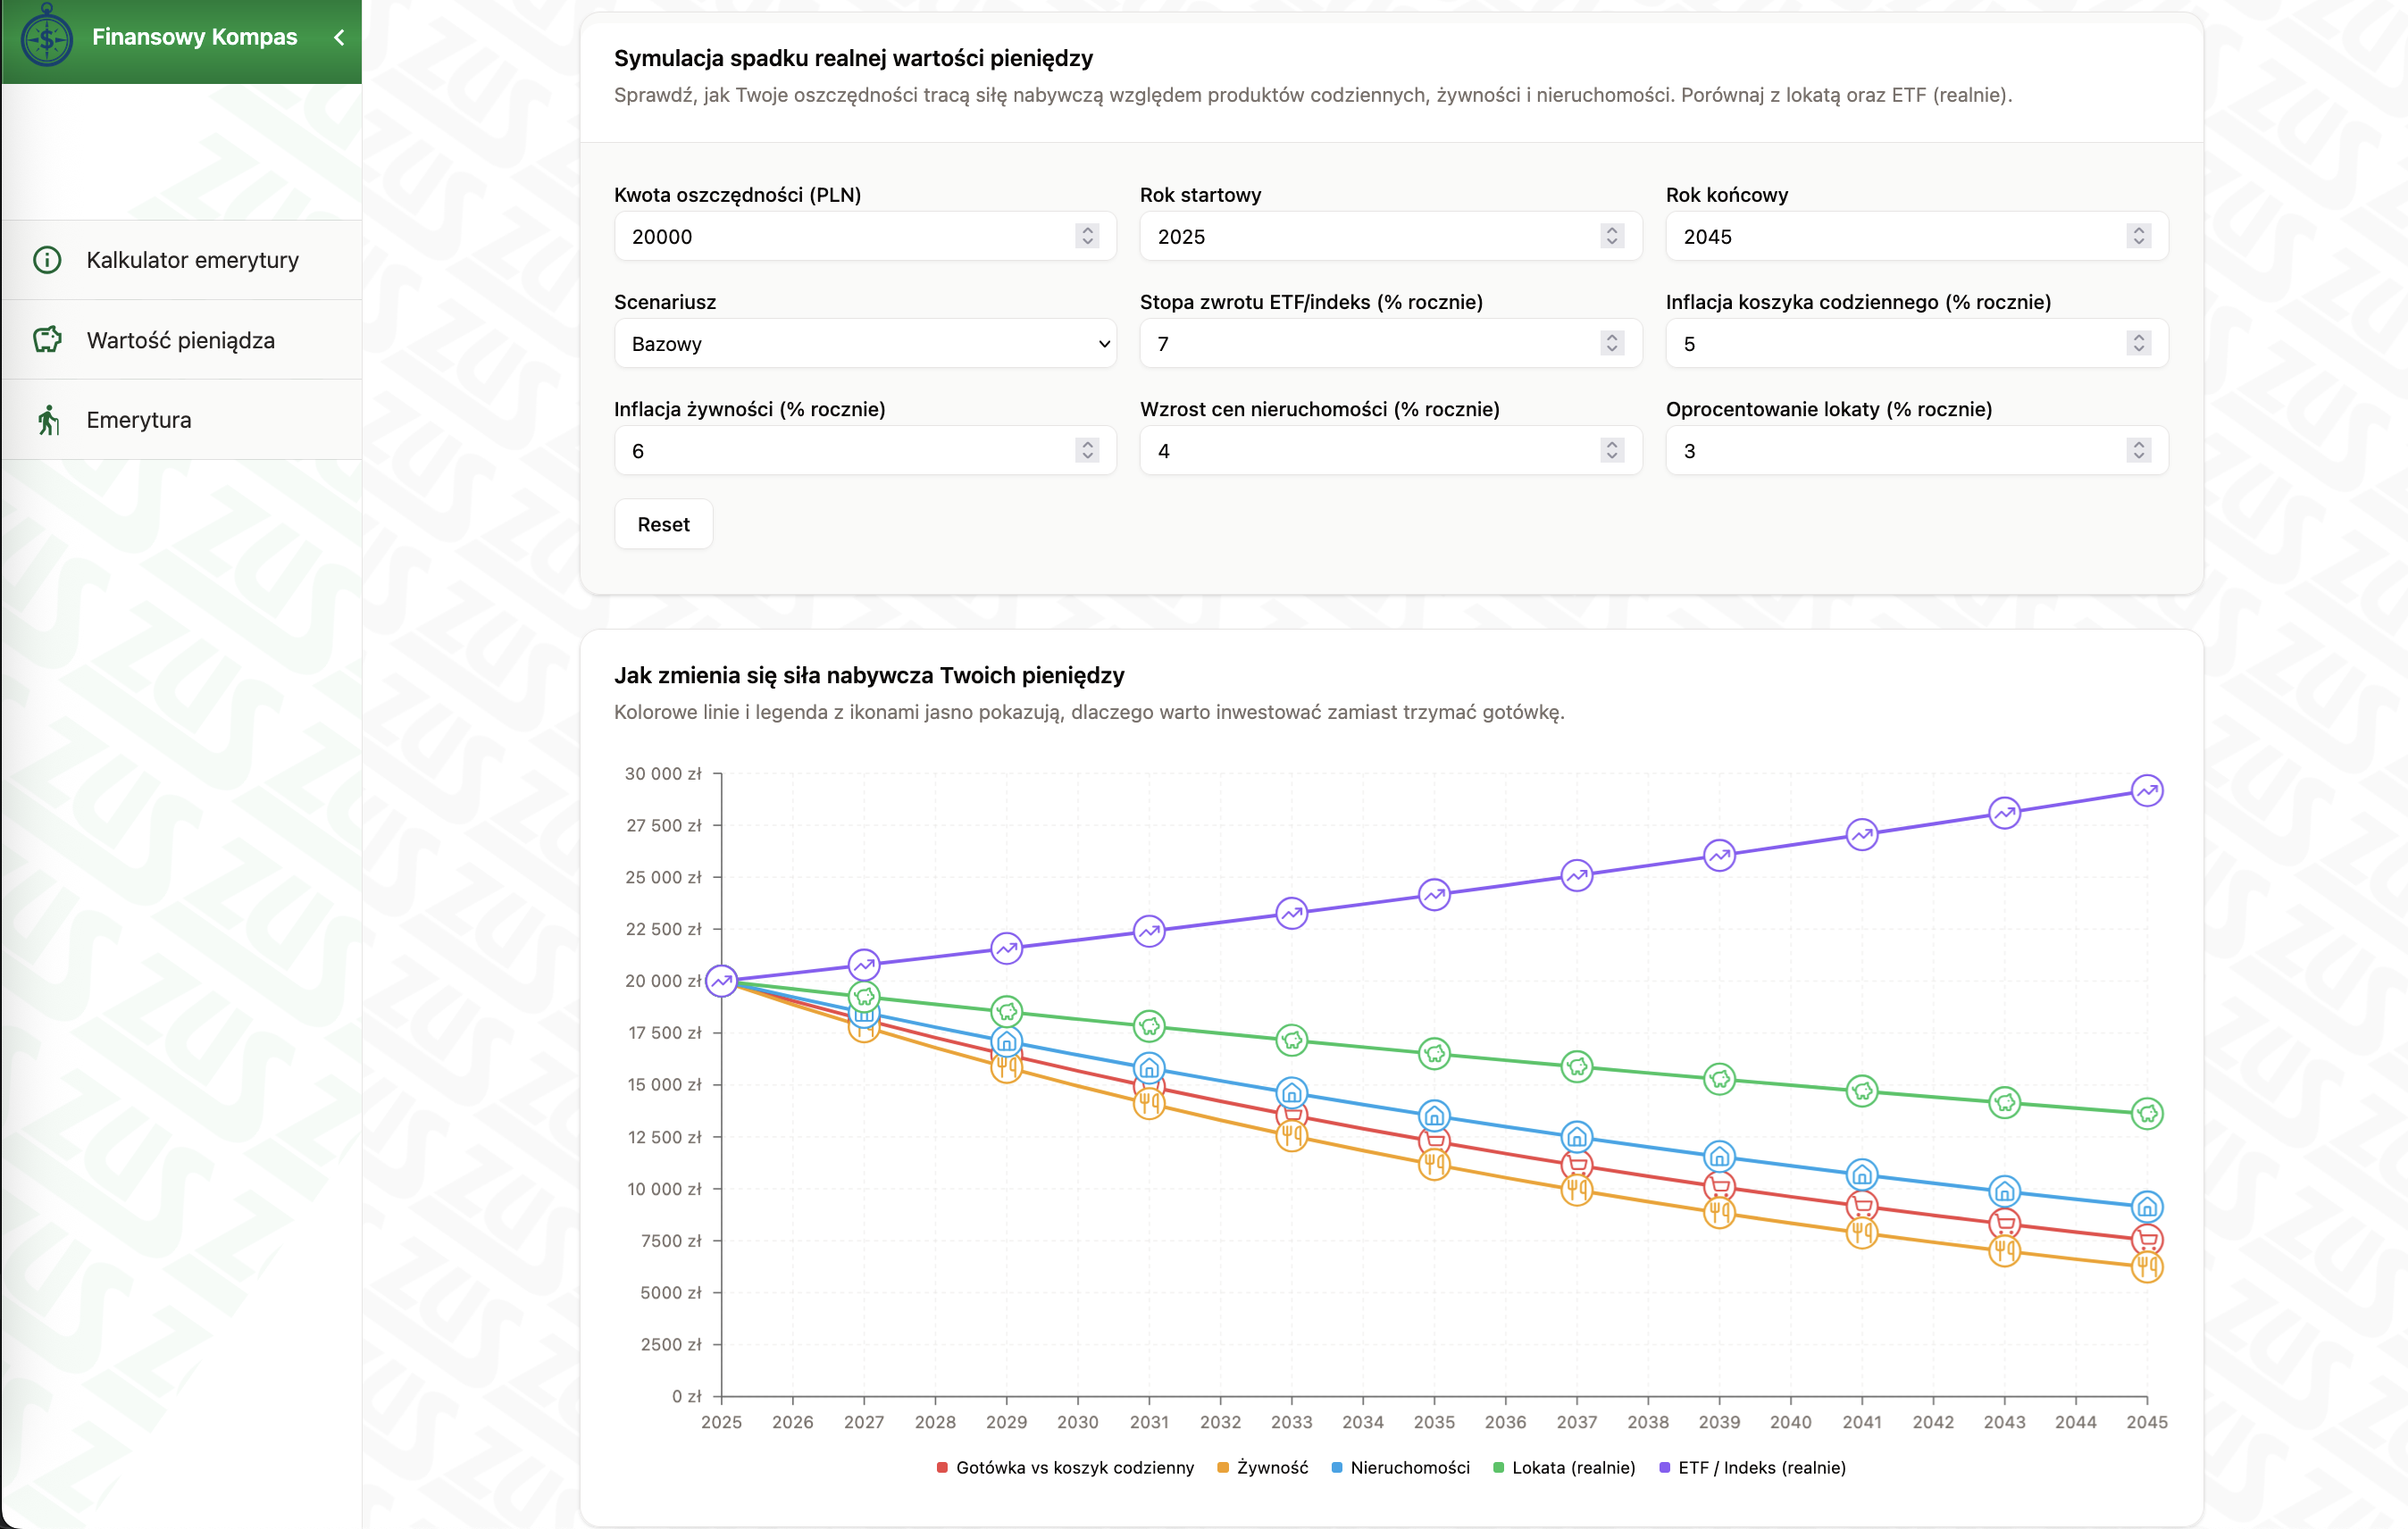
\includegraphics[width=.8\textwidth]{img/module_3_the_value_of_money}
\end{frame}

\begin{frame}[t]{Moduł III}{Wartość pieniądza}
Celem modulu ,,Wartość pieniądza'' jest przede wszystkim ilustracja
i urealnienie pojęcia inflacji młodym ludziom.

\pause Poprzez pokazanie różnych,
w pełni konfigurowalnych scenariuszy użytkownik obserwuje na dynamicznym
wykresie jak szybko spada wartość oszczędności trzymanych na koncie
oszczędnościowym czy lokacie.


\pause Dla porównania wykres zawiera też dane
na temat rosnących cen podstawowych dóbr materialnych: żywności, nieruchomości
oraz przykładowe dane globalnych akcji w formie zdywersyfikowanego funduszu ETF.
\end{frame}

\subsection{Moduł IV --- Rozszerzony kalkulator emerytalny}

\begin{frame}[t]{Moduł IV}{Rozszerzony kalkulator emerytalny}
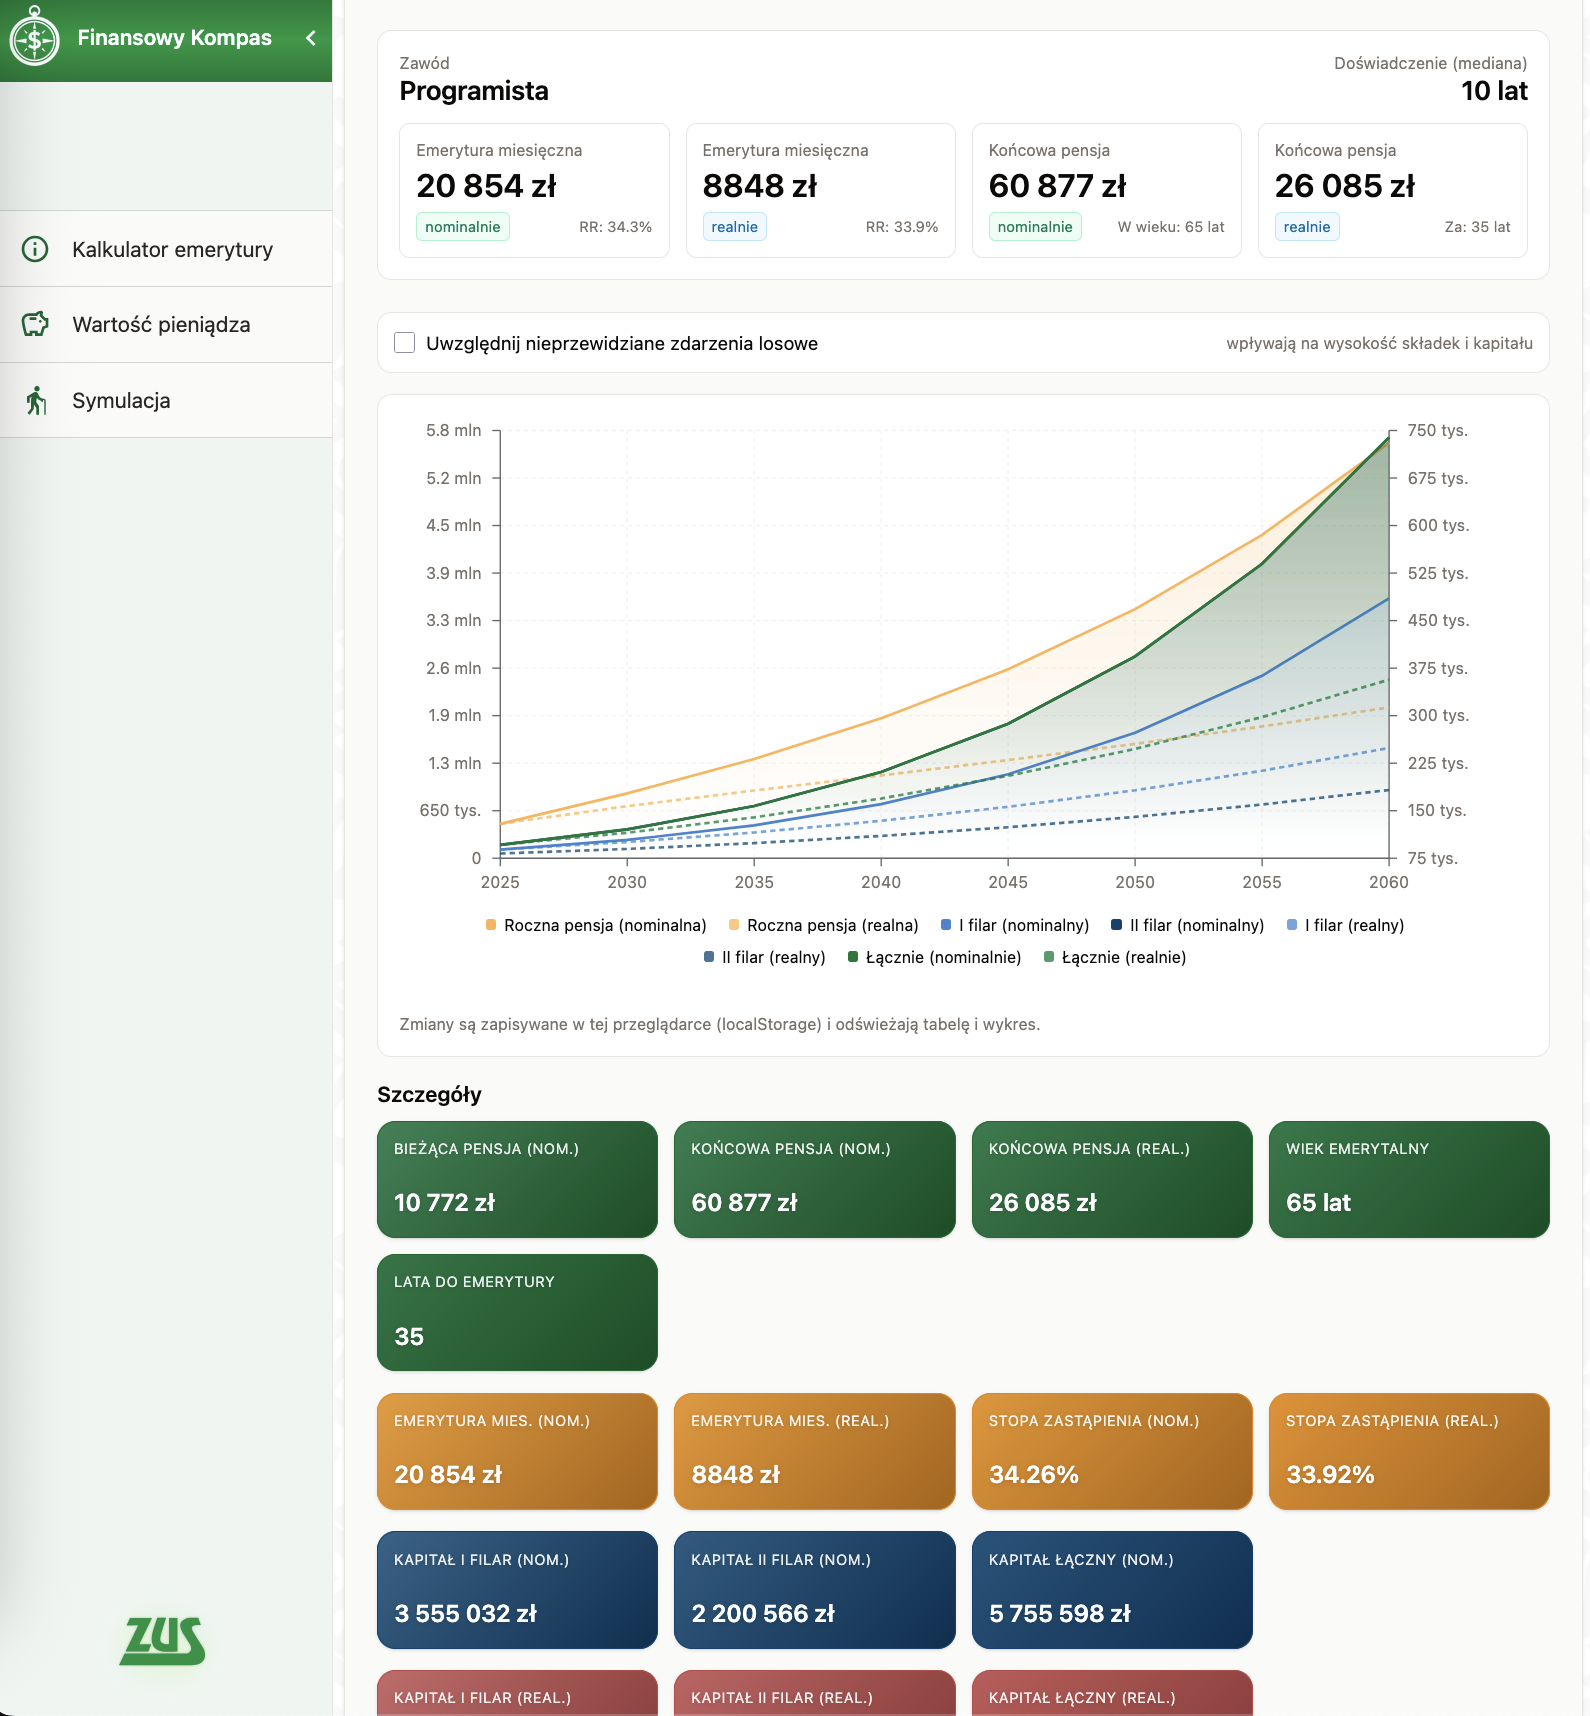
\includegraphics[width=.8\textwidth]{img/module_4_extended_pension_calculator}
\end{frame}

\begin{frame}[t]{Moduł IV}{Rozszerzony kalkulator emerytalny}
W odróżnieniu od modułu II, moduł IV nie tylko wykorzystuje pełnię danych od użytkownika
(wpisanych ręcznie lub wyliczonych z naszych modeli i rozsądnych wartości domyślnych),
ale również ilustruje wszystkie ważne parametry emerytury:

\begin{itemize}
    \pause
    \item wykres, obrazujący pieniądze gromadzone na koncie i subkoncie ZUS przez pozostałe lata aktywności
    zawodowej
    \pause
    \item progresję zarobków, wartości emerytury i tzw. stopę zastąpienia --- realną procentową zmianę
    przychodzu, jakiej nasz użytkownik dozna w momencie przejścia na emeryturę.
\end{itemize}
\end{frame}

\begin{frame}[t]{Moduł IV}{Rozszerzony kalkulator emerytalny}
W odróżnieniu od modułu II, moduł IV nie tylko wykorzystuje pełnię danych od użytkownika
(wpisanych ręcznie lub wyliczonych z naszych modeli i rozsądnych wartości domyślnych),
ale również ilustruje wszystkie ważne parametry emerytury:

\begin{itemize}
    \pause
    \item wykres, obrazujący pieniądze gromadzone na koncie i subkoncie ZUS przez pozostałe lata aktywności
    zawodowej
    \pause
    \item progresję zarobków, wartości emerytury i tzw. stopę zastąpienia --- realną procentową zmianę
    przychodzu, jakiej nasz użytkownik dozna w momencie przejścia na emeryturę.
\end{itemize}
\end{frame}

\subsection{Moduł V --- Symulacja wydarzeń losowych}

\begin{frame}[t]{Moduł V}{Symulacja wydarzeń losowych}
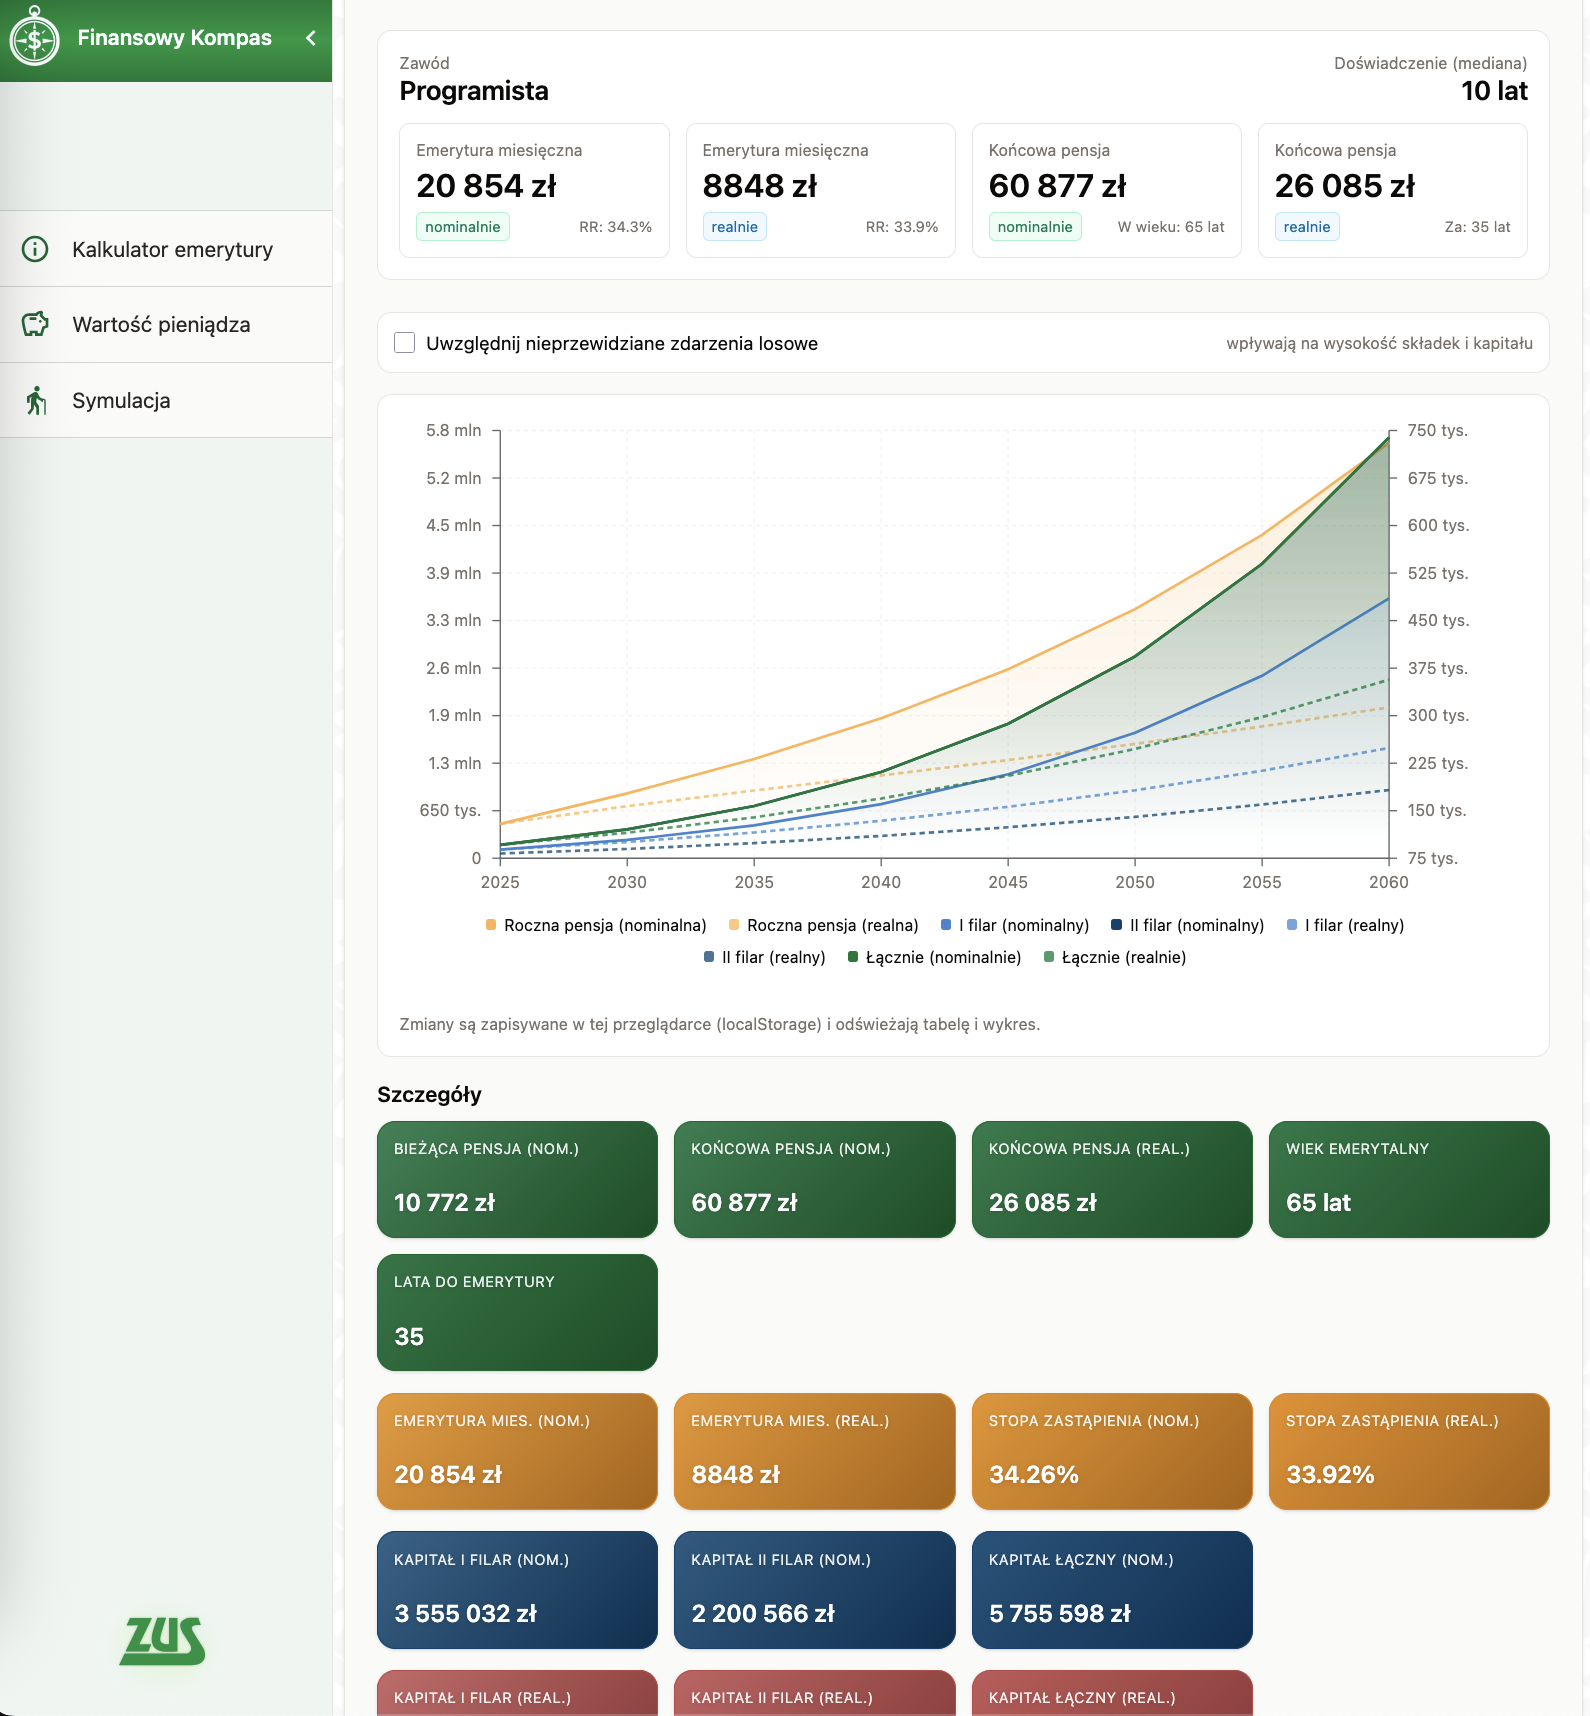
\includegraphics[width=.8\textwidth]{img/module_4_extended_pension_calculator}
\end{frame}

\begin{frame}[t]{Moduł V}{Symulacja wydarzeń losowych}
Osobny, opcjonalny model, który wprowadza zdarzenia losowe
(utrata pracy, choroba, urlop macierzyński itp.)
do wyliczeń w ramach IV modulu (rozszerzonego kalkulatora emerytalnego).

\pause Moduł pozwala użytkownikom zrozumieć głeboki wpływ, jaki wczesne
zaburzenia w ciągłości zatrudnienia i odprowadzania składek potrafią mieć
na końcową emeryturę.
\end{frame}

\subsection{Moduł VI --- Zbieranie danych statystycznych i generowanie raportu .xls}

\begin{frame}[t]{Moduł VI}{Zbieranie danych statystycznych i generowanie raportu .xls}
Choć postanowiliśmy nie dodawać na etapie Hackatonu żadnego modułu do autoryzacji dostępu
i bazy danych, zaimplementowaliśmy prosty moduł zbierania danych statystycznych o użytkownikach
(zgodnie, z wymaganiami zadania) z możliwością pobrania raportu z tymi danymni w formie
pliku Excel.
\end{frame}